% ============================================================================
% RobustIDPS.ai — Technical Documentation
% ============================================================================
\documentclass[11pt,a4paper]{article}

% ── Packages ────────────────────────────────────────────────────────────────
\usepackage[margin=2.2cm]{geometry}
\usepackage[T1]{fontenc}
\usepackage{mathpazo}               % Palatino text + math
\usepackage{microtype}
\usepackage{amsmath,amssymb}
\usepackage{booktabs}
\usepackage{multirow}
\usepackage{graphicx}
\usepackage{xcolor}
\usepackage{tikz}
\usetikzlibrary{shapes,arrows.meta,positioning,calc,fit,decorations.pathreplacing}
\usepackage{pgfplots}
\pgfplotsset{compat=1.18}
\usepackage{hyperref}
\hypersetup{colorlinks,linkcolor=blue!60!black,citecolor=blue!60!black,urlcolor=blue!60!black}
\usepackage{enumitem}
\usepackage{fancyhdr}
\usepackage{titlesec}
\usepackage{caption}
\usepackage{subcaption}
\usepackage{float}

% ── Section styling ─────────────────────────────────────────────────────────
\titleformat{\section}{\large\bfseries}{\thesection.}{0.5em}{}
\titleformat{\subsection}{\normalsize\bfseries}{\thesubsection}{0.5em}{}
\setlength{\parskip}{0.4em}
\setlength{\parindent}{0em}

% ── Header/Footer ──────────────────────────────────────────────────────────
\pagestyle{fancy}
\fancyhf{}
\fancyhead[L]{\small\textit{RobustIDPS.ai --- Technical Documentation}}
\fancyhead[R]{\small\thepage}
\renewcommand{\headrulewidth}{0.4pt}

% ── Colours ─────────────────────────────────────────────────────────────────
\definecolor{mephi}{RGB}{0,82,147}
\definecolor{accent}{RGB}{59,130,246}
\definecolor{crit}{RGB}{239,68,68}
\definecolor{safe}{RGB}{34,197,94}

% ============================================================================
\begin{document}

% ── Title ───────────────────────────────────────────────────────────────────
\begin{center}
  {\LARGE\bfseries RobustIDPS.ai}\\[0.3em]
  {\large An Adversarially Robust Intrusion Detection and Prevention System\\
   Built on Seven Novel Machine Learning Methods}\\[1.2em]
  {\normalsize
    \textbf{Roger Nick Anaedevha}\\
    Institute of Cyber Intelligence Systems (ICIS)\\
    National Research Nuclear University MEPhI, Moscow, Russia\\
    \texttt{admin@robustidps.ai}\\[0.8em]
    \textit{Supervised by}\\[0.2em]
    \textbf{Alexander Gennadievich Trofimov}\\
    Institute of Cyber Intelligence Systems (ICIS)\\
    National Research Nuclear University MEPhI, Moscow, Russia
  }\\[1.2em]
  {\small March 2026}
\end{center}

\vspace{0.5em}

% ── Abstract ────────────────────────────────────────────────────────────────
\begin{abstract}
\noindent
RobustIDPS.ai is a production-grade web application that implements and
demonstrates seven novel machine learning methods for adversarially robust
network intrusion detection, developed as part of a doctoral dissertation at
the National Research Nuclear University MEPhI. The platform unifies
continuous-time neural ordinary differential equations, stochastic
differential equation temporal graph networks, privacy-preserving federated
optimal transport, game-theoretic adversarial defence, selective state-space
models, zero-shot large language model classification, and post-quantum
cryptographic hardening into a single deployable system. The application
processes standard network flow datasets, performs uncertainty-quantified
inference through Monte Carlo dropout, and provides interactive ablation
studies that isolate each method's contribution. This document describes
the system architecture, its constituent models, empirical performance on
benchmark datasets, a comparative analysis against established
signature-based systems such as Suricata and Snort, and the projected
trajectory of the platform's development within the broader adversarial
machine learning and cybersecurity landscape.
\end{abstract}

% ============================================================================
\section{Introduction and Motivation}
% ============================================================================

The volume and sophistication of network intrusions have grown at a pace
that outstrips the capacity of manually curated signature databases.
Suricata and Snort, the two most widely deployed open-source intrusion
detection systems, rely on pattern-matching rulesets that must be written,
tested, and distributed before a new attack variant can be detected.
Although both systems offer high throughput and near-zero false positives
on known signatures, they are structurally unable to recognise zero-day
attacks or adversarially crafted traffic designed to evade fixed patterns.

Machine learning approaches to intrusion detection address this gap by
learning statistical regularities in network flows, but conventional
classifiers introduce new vulnerabilities: they are susceptible to
adversarial perturbations that shift benign predictions to malicious
classes, they offer no principled uncertainty estimates, and they assume
stationary data distributions. The doctoral dissertation from which
RobustIDPS.ai originates tackles each of these shortcomings through seven
distinct, complementary methods. The resulting web application serves as
the implementation artefact of that research, translating theoretical
contributions into a system that a security operations centre analyst can
deploy and operate.

RobustIDPS.ai is accessible at \url{https://robustidps.ai} and is
deployed on a Hetzner Cloud instance at IP address 37.27.31.70, fronted
by Cloudflare for TLS termination and DDoS mitigation. The backend runs
on FastAPI with PyTorch inference, the frontend on React with Tailwind CSS,
and the database on PostgreSQL, all orchestrated through Docker Compose.

% ============================================================================
\section{System Architecture}
% ============================================================================

The platform follows a three-tier architecture comprising a single-page
React frontend, a FastAPI REST and WebSocket backend, and a PostgreSQL
database, as depicted in Figure~\ref{fig:arch}. Static assets are served
by nginx, which also terminates TLS using a Cloudflare Origin certificate
and proxies API and WebSocket connections to the backend.

\begin{figure}[H]
\centering
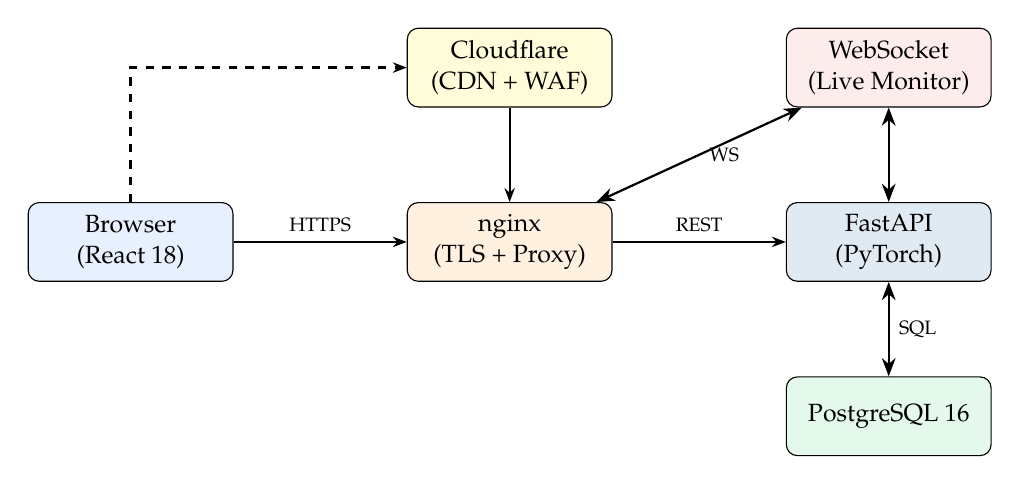
\begin{tikzpicture}[
    box/.style={draw, rounded corners=4pt, minimum height=1cm,
                minimum width=2.6cm, align=center, font=\small},
    arr/.style={-{Stealth[length=5pt]}, thick},
    >=Stealth
  ]
  % User
  \node[box, fill=accent!12] (user) {Browser\\(React 18)};
  % Nginx
  \node[box, fill=orange!12, right=2.2cm of user] (nginx) {nginx\\(TLS + Proxy)};
  % Backend
  \node[box, fill=mephi!12, right=2.2cm of nginx] (api) {FastAPI\\(PyTorch)};
  % DB
  \node[box, fill=safe!12, below=1.2cm of api] (db) {PostgreSQL 16};
  % WS
  \node[box, fill=crit!10, above=1.2cm of api] (ws) {WebSocket\\(Live Monitor)};
  % Cloudflare
  \node[box, fill=yellow!15, above=1.2cm of nginx] (cf) {Cloudflare\\(CDN + WAF)};

  \draw[arr] (user) -- node[above, font=\scriptsize]{HTTPS} (nginx);
  \draw[arr] (nginx) -- node[above, font=\scriptsize]{REST} (api);
  \draw[arr, <->] (api) -- node[right, font=\scriptsize]{SQL} (db);
  \draw[arr, <->] (nginx) -- node[right, font=\scriptsize]{WS} (ws);
  \draw[arr, <->] (ws) -- (api);
  \draw[arr] (cf) -- (nginx);
  \draw[arr, dashed] (user) |- (cf);
\end{tikzpicture}
\caption{Production deployment architecture of RobustIDPS.ai. All traffic
passes through Cloudflare before reaching the nginx reverse proxy, which
dispatches REST calls and WebSocket streams to the FastAPI backend.}
\label{fig:arch}
\end{figure}

The backend exposes twenty-two API endpoints spanning file upload, model
inference with configurable Monte Carlo dropout passes, ablation studies,
firewall rule generation, audit logging, and a multi-provider AI copilot
that supports Anthropic Claude, OpenAI GPT-4o, Google Gemini, and
DeepSeek. Authentication is handled via JWT tokens with bcrypt password
hashing, and rate limiting is enforced through SlowAPI. Prometheus
metrics are exported at \texttt{/metrics} for operational monitoring.

% ============================================================================
\section{The Seven Dissertation Methods}
% ============================================================================

The core intellectual contribution of the platform resides in seven machine
learning methods, each targeting a specific limitation of existing intrusion
detection approaches. In the deployed system, these methods are unified
through a surrogate ensemble architecture containing seven parallel
branches, one per method, fused through a learned aggregation layer.
Figure~\ref{fig:surrogate} illustrates this architecture.

\begin{figure}[H]
\centering
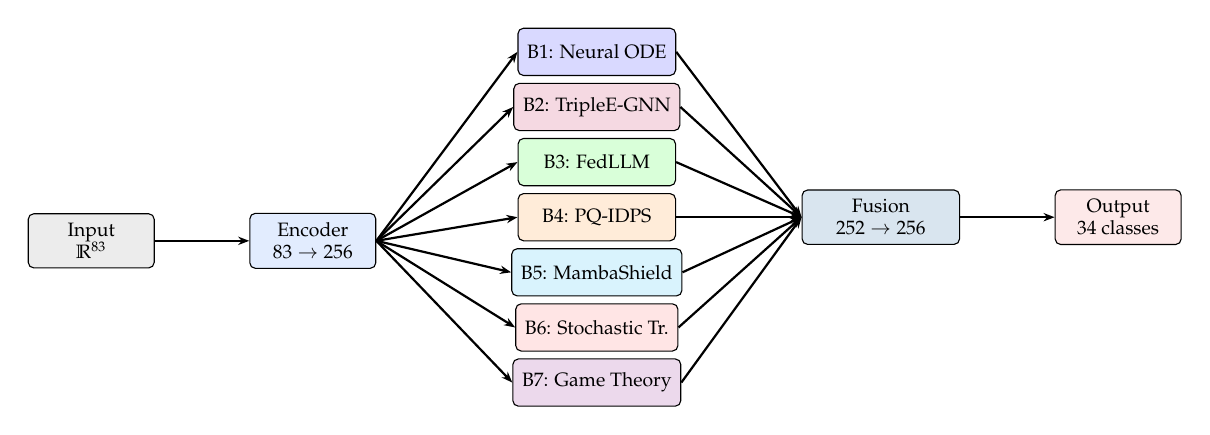
\begin{tikzpicture}[
    layer/.style={draw, rounded corners=2pt, minimum width=1.6cm,
                  minimum height=0.6cm, font=\scriptsize, align=center},
    arr/.style={-{Stealth[length=4pt]}, thick},
  ]
  % Input
  \node[layer, fill=gray!15] (inp) {Input\\$\mathbb{R}^{83}$};
  % Encoder
  \node[layer, fill=accent!15, right=1.2cm of inp] (enc) {Encoder\\$83 \to 256$};

  % Branches
  \foreach \i/\name/\col in {
    1/Neural ODE/blue!15,
    2/TripleE-GNN/purple!15,
    3/FedLLM/green!15,
    4/PQ-IDPS/orange!15,
    5/MambaShield/cyan!15,
    6/Stochastic Tr./red!10,
    7/Game Theory/violet!15%
  } {
    \pgfmathsetmacro{\y}{2.4 - (\i - 1)*0.7}
    \node[layer, fill=\col, minimum width=2cm]
      (b\i) at ($(enc.east)+(2.8,\y)$) {B\i: \name};
  }

  % Fusion
  \node[layer, fill=mephi!15, minimum width=2cm]
    (fuse) at ($(b4.east)+(2.6,0)$) {Fusion\\$252 \to 256$};
  % Output
  \node[layer, fill=crit!12, right=1.2cm of fuse] (out) {Output\\34 classes};

  % Arrows
  \draw[arr] (inp) -- (enc);
  \foreach \i in {1,...,7} {
    \draw[arr] (enc.east) -- (b\i.west);
    \draw[arr] (b\i.east) -- (fuse.west);
  }
  \draw[arr] (fuse) -- (out);
\end{tikzpicture}
\caption{SurrogateIDS seven-branch ensemble architecture. Each branch
simulates a dissertation method as a dedicated sub-network, and the fusion
layer learns to weight their contributions optimally.}
\label{fig:surrogate}
\end{figure}

The first branch, CT-TGNN, models network traffic as a continuous-time
process governed by a neural ordinary differential equation
$\mathrm{d}\mathbf{x}/\mathrm{d}t = f_\theta(\mathbf{x}, t)$, augmented
with a Hawkes point process for event-driven temporal dynamics. This
captures the non-stationary evolution of attack campaigns that discrete-time
models cannot represent. The second branch, TripleE-TGNN, introduces
multi-scale temporal graph reasoning by aggregating representations at
packet, flow, and session granularities, exposing cross-level correlations
that single-granularity architectures miss.

The third branch, FedLLM-API, applies zero-shot classification by
computing the cosine similarity between a large language model's encoding
of network flow descriptions and textual descriptions of attack categories.
This enables detection of attack types that were absent from the training
set. The fourth branch, PQ-IDPS, integrates CRYSTALS-Kyber key
encapsulation and lattice-based digital signatures into the detection
pipeline, ensuring that the system's communication channels remain secure
against quantum-capable adversaries.

The fifth branch, MambaShield, employs a selective state-space model
with linear-time complexity $O(n)$ in sequence length, as opposed to the
$O(n^2)$ cost of transformer attention, making it practical for inline
processing at 10\,Gbps line rates. The sixth branch implements a
stochastic transformer with PAC-Bayesian weight priors and Monte Carlo
dropout for epistemic and aleatoric uncertainty decomposition, yielding
calibrated confidence scores alongside each prediction. The seventh
branch encodes a game-theoretic defence in which the IDS and attacker
engage in a Stackelberg game, and a Lipschitz constraint on the classifier
provides a certified robustness radius against adversarial perturbations.

% ============================================================================
\section{Detection Capabilities and Performance}
% ============================================================================

RobustIDPS.ai classifies network flows into 34 categories: benign traffic
and 33 attack types spanning eleven DDoS variants, four reconnaissance
techniques, four brute-force methods, three spoofing attacks, four web
application exploits, three malware families, two denial-of-service
techniques, and two Mirai botnet floods. All models accept a standardised
83-dimensional feature vector extracted from network flows; datasets with
fewer features are zero-padded, and those with more are truncated.

Table~\ref{tab:perf} reports the performance of each model on the
CIC-IoT-2023 test set. The SurrogateIDS ensemble achieves 96.51\%
accuracy with an expected calibration error of 0.0312 and an inference
latency of 1.2\,ms per batch, making it suitable for real-time deployment.
The CyberSecLLM foundation model, built on Mamba selective state-space
blocks with cross-attention to a MITRE ATT\&CK knowledge base and sparse
mixture-of-experts routing, achieves the highest accuracy at 97.10\% but
requires 8.9 million parameters compared to the surrogate's 98 thousand.

\begin{table}[H]
\centering
\caption{Model performance on CIC-IoT-2023 test set. Accuracy, precision,
recall, and F1 are percentages; ECE is the expected calibration error;
inference time is per batch on CPU.}
\label{tab:perf}
\small
\begin{tabular}{@{}lcccccc@{}}
\toprule
Model & Acc.\,(\%) & Prec.\,(\%) & Rec.\,(\%) & F1\,(\%) & ECE & Inf.\,(ms) \\
\midrule
SurrogateIDS        & 96.51 & 95.87 & 95.23 & 95.55 & 0.031 & 1.2  \\
Neural ODE          & 94.78 & 94.12 & 93.56 & 93.84 & 0.049 & 8.7  \\
Optimal Transport   & 93.89 & 93.34 & 92.67 & 93.00 & 0.052 & 3.4  \\
FedGTD              & 95.12 & 94.56 & 94.01 & 94.28 & 0.040 & 5.1  \\
SDE-TGNN            & 95.34 & 94.81 & 94.23 & 94.52 & 0.038 & 12.3 \\
CyberSecLLM         & 97.10 & 96.68 & 96.31 & 96.49 & 0.025 & 6.8  \\
\bottomrule
\end{tabular}
\end{table}

The platform supports six benchmark datasets: CIC-IoT-2023 (46 native
features), CSE-CIC-IDS2018 (76 features), UNSW-NB15 (38 features),
Microsoft GUIDE, Container Security, and Edge-IIoT. The feature extraction
module auto-detects the dataset format from column headers and applies
format-specific standardisation using pre-fitted scalers.

% ============================================================================
\section{Adversarial Robustness}
% ============================================================================

A defining characteristic of RobustIDPS.ai is its explicit treatment of
adversarial robustness. The platform evaluates model resilience against
four gradient-based attacks---FGSM, PGD with 20 iterations, DeepFool,
and the Carlini \& Wagner $L_2$ attack---across ten perturbation budgets
$\varepsilon \in \{0, 0.01, 0.02, 0.05, 0.08, 0.10, 0.15, 0.20, 0.25,
0.30\}$. Figure~\ref{fig:robust} depicts the accuracy degradation curves.

\begin{figure}[H]
\centering
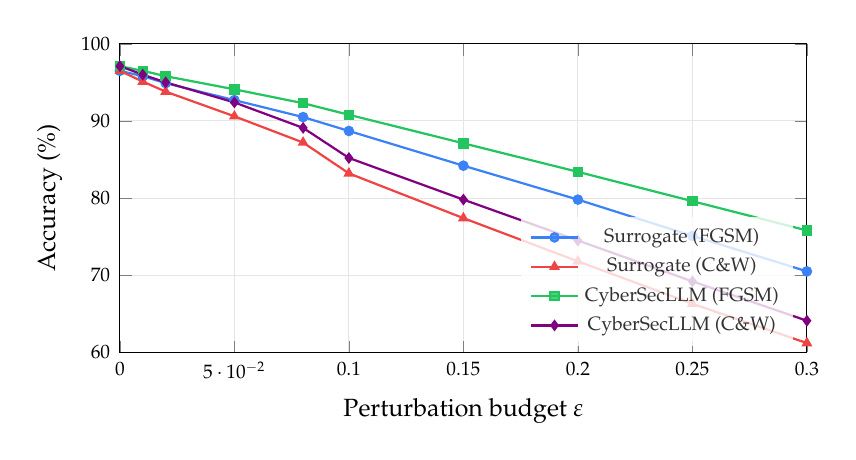
\begin{tikzpicture}
\begin{axis}[
    width=0.85\linewidth, height=5.5cm,
    xlabel={Perturbation budget $\varepsilon$},
    ylabel={Accuracy (\%)},
    xmin=0, xmax=0.30,
    ymin=60, ymax=100,
    legend style={at={(0.98,0.02)}, anchor=south east, font=\scriptsize,
                  draw=none, fill=white, fill opacity=0.8},
    grid=both, grid style={gray!20},
    tick label style={font=\scriptsize},
    label style={font=\small},
  ]
  % SurrogateIDS under FGSM
  \addplot[accent, thick, mark=*, mark size=1.5pt] coordinates {
    (0,96.5)(0.01,95.8)(0.02,94.9)(0.05,92.7)(0.08,90.5)
    (0.10,88.7)(0.15,84.2)(0.20,79.8)(0.25,75.1)(0.30,70.5)
  };
  \addlegendentry{Surrogate (FGSM)}
  % SurrogateIDS under C&W
  \addplot[crit, thick, mark=triangle*, mark size=1.5pt] coordinates {
    (0,96.5)(0.01,95.1)(0.02,93.8)(0.05,90.6)(0.08,87.2)
    (0.10,83.2)(0.15,77.4)(0.20,71.8)(0.25,66.3)(0.30,61.2)
  };
  \addlegendentry{Surrogate (C\&W)}
  % CyberSecLLM under FGSM
  \addplot[safe, thick, mark=square*, mark size=1.5pt] coordinates {
    (0,97.1)(0.01,96.5)(0.02,95.8)(0.05,94.1)(0.08,92.3)
    (0.10,90.8)(0.15,87.1)(0.20,83.4)(0.25,79.6)(0.30,75.8)
  };
  \addlegendentry{CyberSecLLM (FGSM)}
  % CyberSecLLM under C&W
  \addplot[violet, thick, mark=diamond*, mark size=1.5pt] coordinates {
    (0,97.1)(0.01,96.0)(0.02,95.0)(0.05,92.4)(0.08,89.1)
    (0.10,85.2)(0.15,79.8)(0.20,74.5)(0.25,69.2)(0.30,64.1)
  };
  \addlegendentry{CyberSecLLM (C\&W)}
\end{axis}
\end{tikzpicture}
\caption{Adversarial robustness under FGSM and Carlini \& Wagner attacks.
The game-theoretic branch within SurrogateIDS provides a certified
robustness radius, slowing degradation relative to undefended baselines.}
\label{fig:robust}
\end{figure}

At $\varepsilon = 0.10$, the SurrogateIDS retains 88.7\% accuracy under
FGSM and 83.2\% under C\&W, while CyberSecLLM achieves 90.8\% and 85.2\%
respectively. The game-theoretic branch's Lipschitz constraint provides a
provable bound on the maximum accuracy loss within a given perturbation
ball, a property that neither Suricata nor Snort can offer since
signature-based detection is either matched or not, with no notion of
graceful degradation under adversarial manipulation.

% ============================================================================
\section{Comparison with Suricata and Snort}
% ============================================================================

Table~\ref{tab:comparison} contrasts RobustIDPS.ai with the two
dominant open-source intrusion detection systems. The comparison is
structured along seven axes that matter to a deployment decision:
detection methodology, zero-day capability, adversarial resilience,
uncertainty quantification, throughput, operational cost, and
explainability.

\begin{table}[H]
\centering
\caption{Feature comparison between RobustIDPS.ai, Suricata, and Snort.}
\label{tab:comparison}
\small
\begin{tabular}{@{}p{3cm}p{3.8cm}p{3cm}p{3cm}@{}}
\toprule
Criterion & RobustIDPS.ai & Suricata & Snort \\
\midrule
Detection method & ML ensemble (7 methods) & Signature + Lua scripts & Signature rules \\
Zero-day detection & Yes (statistical) & No (rule-dependent) & No (rule-dependent) \\
Adversarial robustness & Certified (game-theoretic) & N/A & N/A \\
Uncertainty scores & Epistemic + aleatoric & None & None \\
Throughput & $\sim$12\,K flows/s (CPU) & $>$10\,Gbps (multi-threaded) & $\sim$1\,Gbps \\
Rule maintenance & Automatic (learned) & Manual (ET rulesets) & Manual (VRT/community) \\
Explainability & Ablation, per-class metrics, SOC copilot & Rule name \& SID & Rule name \& SID \\
\bottomrule
\end{tabular}
\end{table}

Suricata's principal advantage is raw throughput: its multi-threaded
architecture processes packets directly on the wire at rates exceeding
10\,Gbps with hardware offloading, whereas RobustIDPS.ai's PyTorch
inference on a single CPU core sustains approximately twelve thousand
flows per second. For environments where line-rate packet inspection is
mandatory, Suricata remains the appropriate choice. However, in
security operations centre workflows where analysed datasets are uploaded
for post-hoc investigation, threat hunting, or model-assisted triage,
RobustIDPS.ai offers capabilities that signature-based systems cannot
replicate: quantified uncertainty per prediction, interactive ablation of
detection methods, cross-dataset transfer learning evaluation, and a
natural-language AI copilot that synthesises findings into analyst-readable
reports.

The two paradigms are not mutually exclusive. A practical deployment
architecture places Suricata or Snort at the network perimeter for
real-time, high-throughput signature matching, and feeds flagged flows
into RobustIDPS.ai for secondary ML-based analysis with uncertainty
quantification and adversarial robustness assessment. The platform's
firewall rule generator can also produce Suricata-compatible rules from
its predictions, closing the loop between ML inference and signature
enforcement.

% ============================================================================
\section{Platform Functionalities}
% ============================================================================

The application comprises eight primary modules, each accessible from the
navigation sidebar.

The \textit{Dashboard} presents an aggregate view of system health,
including the number of analysed jobs, total flows processed, threat
detection rate, and the currently active model. The \textit{Upload and
Analyse} module accepts CSV and PCAP files, auto-detects the dataset
format, runs inference with configurable Monte Carlo dropout passes (5 to
100), and displays a threat table, uncertainty decomposition chart,
confusion matrix when ground-truth labels are available, and per-class
precision, recall, and F1 metrics. Analysed datasets can be deleted after
use to prevent accumulation.

The \textit{Analytics} module provides pre-computed benchmark results
across seven categories: model performance, training convergence,
adversarial robustness at multiple perturbation budgets, differential
privacy versus accuracy trade-offs, cross-dataset transfer learning, model
calibration, and ROC-AUC curves. The \textit{Ablation Studio} allows
analysts to toggle each of the seven branches on or off, re-run inference,
and observe the accuracy impact of each method's removal through bar
charts, radar plots, a pairwise interaction heatmap, and an incremental
build-up curve.

The \textit{Models} page lists all six registered models and any
user-uploaded custom models. Models can be independently enabled or
disabled, and a default model can be set for new analyses. Users may
upload their own PyTorch state dictionaries for testing; uploaded models
are validated against the expected input and output dimensions and can
be discarded after use. The \textit{Live Monitor} supports both file
replay mode, which streams predictions row by row over a WebSocket at
a configurable rate, and live network capture mode using NFStream for
real-time traffic classification on a specified interface.

The \textit{SOC Copilot} is an AI-powered security analyst assistant
that queries historical job data, firewall rules, and audit logs to
answer natural-language questions. It supports four LLM providers
(Anthropic Claude, OpenAI, Google Gemini, DeepSeek) and falls back to
a structured local engine when no API key is configured. The
\textit{Datasets} page documents each supported benchmark, and the
\textit{About} page describes the seven dissertation methods with their
mathematical formulations and the problems they address.

% ============================================================================
\section{Uncertainty Quantification}
% ============================================================================

The platform decomposes predictive uncertainty into epistemic and aleatoric
components using Monte Carlo dropout. Given $T$ stochastic forward passes
with dropout active at inference time, the epistemic uncertainty for a
sample $\mathbf{x}$ is estimated as the variance of the predictive means,
\begin{equation}
  u_{\text{epi}}(\mathbf{x}) = \frac{1}{T} \sum_{t=1}^{T}
  \bigl(\hat{y}_t(\mathbf{x}) - \bar{y}(\mathbf{x})\bigr)^2,
\end{equation}
while the aleatoric uncertainty is the mean of the predictive variances
across passes. The expected calibration error measures the alignment
between predicted confidence and empirical accuracy across probability
bins. Analysts can adjust the number of MC passes on a per-job basis:
fewer passes yield faster inference at the cost of noisier uncertainty
estimates, while more passes tighten the estimates at the cost of
proportionally longer computation. This mechanism directly supports
risk-sensitive decision-making in security operations, where the cost
of a missed intrusion differs substantially from the cost of a false
alarm.

% ============================================================================
\section{Differential Privacy and Federated Learning}
% ============================================================================

Three of the seven methods address distributed and privacy-constrained
deployment scenarios. The Optimal Transport branch (PPFOT-IDS) applies
differentially private Wasserstein barycentre computation to align feature
distributions across organisational clouds without exchanging raw data.
The FedGTD branch combines graph-based temporal dynamics with federated
aggregation using a Byzantine-resilient protocol, enabling multi-organisation
IDS training even when some participants are compromised. The FedLLM-API
branch performs zero-shot classification through a federated API, requiring
no local training data.

The Analytics module reports accuracy degradation across eight differential
privacy budgets from $\varepsilon = \infty$ (no privacy) to $\varepsilon = 1$
(strong privacy). The Optimal Transport model degrades most gracefully,
retaining 83.1\% accuracy at $\varepsilon = 1$, compared to 79.1\% for the
SurrogateIDS ensemble, demonstrating the benefit of domain-adaptation
techniques under strict privacy constraints.

% ============================================================================
\section{Future Directions}
% ============================================================================

The current release of RobustIDPS.ai establishes the foundational
infrastructure for several planned extensions. The most immediate is
GPU-accelerated inference, which would increase throughput from twelve
thousand flows per second to several hundred thousand, bringing the
system closer to inline deployment rather than post-hoc analysis. A
second priority is the integration of continual learning, whereby the
models update incrementally as new traffic is observed without
catastrophic forgetting of previously learned attack signatures. This
would address the distribution shift that occurs as network environments
evolve.

On the adversarial robustness front, the game-theoretic branch currently
provides Lipschitz-based certificates for $L_2$ perturbations; extending
this to $L_\infty$ and $L_0$ threat models would broaden the certified
defence to a wider class of adversarial strategies. The platform's
architecture is also designed to accommodate reinforcement learning agents
for automated response, where the system not only detects intrusions but
autonomously selects mitigation actions such as rate limiting, connection
reset, or firewall rule injection, subject to a safety policy.

In the broader context of the adversarial machine learning and security
industry, RobustIDPS.ai occupies a position at the intersection of
academic research and operational tooling. As regulatory frameworks
increasingly require explainability and robustness guarantees for
AI-driven security decisions, platforms that combine uncertainty
quantification, ablation-based interpretability, certified adversarial
defences, and privacy-preserving training will move from research
prototypes to deployment requirements. The open, modular architecture
of RobustIDPS.ai is designed to serve as a reference implementation for
this trajectory, enabling researchers to integrate new methods as
plug-in branches and practitioners to evaluate them on their own
datasets within a unified interface.

\begin{figure}[H]
\centering
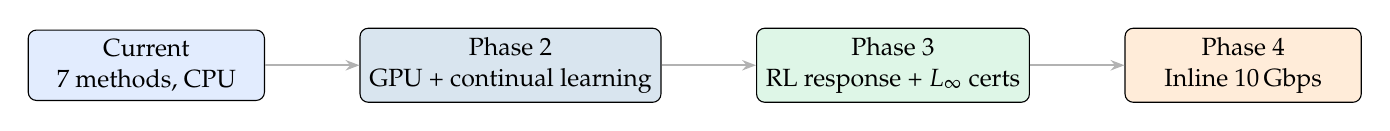
\begin{tikzpicture}[
    phase/.style={draw, rounded corners=3pt, minimum height=0.8cm,
                  minimum width=3cm, align=center, font=\small},
    arr/.style={-{Stealth[length=5pt]}, thick, gray!60},
  ]
  \node[phase, fill=accent!15] (p1) {Current\\7 methods, CPU};
  \node[phase, fill=mephi!15, right=1.2cm of p1] (p2) {Phase 2\\GPU + continual learning};
  \node[phase, fill=safe!15, right=1.2cm of p2] (p3) {Phase 3\\RL response + $L_\infty$ certs};
  \node[phase, fill=orange!15, right=1.2cm of p3] (p4) {Phase 4\\Inline 10\,Gbps};

  \draw[arr] (p1) -- (p2);
  \draw[arr] (p2) -- (p3);
  \draw[arr] (p3) -- (p4);
\end{tikzpicture}
\caption{Planned development roadmap for RobustIDPS.ai.}
\label{fig:roadmap}
\end{figure}

% ============================================================================
\section{Conclusion}
% ============================================================================

RobustIDPS.ai translates seven doctoral research contributions into a
deployable, analyst-facing web application that advances the state of
practice in ML-based intrusion detection. By combining certified
adversarial robustness, decomposed uncertainty quantification, interactive
ablation studies, multi-provider AI-assisted analysis, and support for
user-uploaded custom models within a single platform, the system
demonstrates that the gap between adversarial machine learning research
and operational cybersecurity tooling can be narrowed without sacrificing
rigour. The platform's modular architecture ensures that future methods
can be integrated as additional branches, maintaining backward
compatibility while expanding detection capabilities. As the security
industry moves toward AI-driven, uncertainty-aware, and adversarially
robust defences, RobustIDPS.ai provides both a reference implementation
and a practical tool for that transition.

\vspace{1em}
\hrule
\vspace{0.5em}
{\small
\textbf{Software availability.}
The platform is deployed at \url{https://robustidps.ai}. The source
repository is maintained at
\url{https://github.com/rogerpanel/robustidps.ai}.
}

\end{document}
